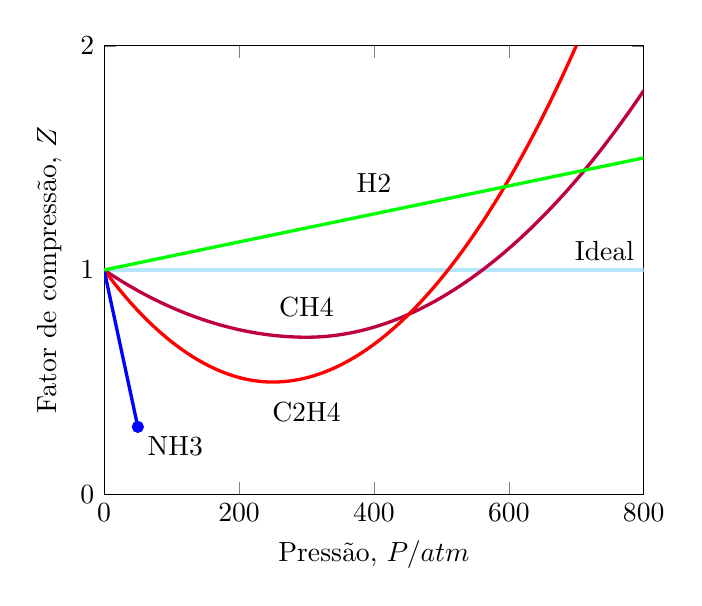
\begin{tikzpicture}
    \begin{axis}
        [
            grid = none,
            xlabel = {Pressão, $P/\unit{atm}$},
            ylabel = {Fator de compressão, $Z$},
            xmin = 0, xmax = 800,
            ymin = 0, ymax = 2,
            ytick = {0, 1, 2},  
            domain = 0:800,
        ]
        \draw [cyan!30, very thick] (axis cs:0, 1) -- (axis cs:800, 1);
        \node [anchor = south east] at (axis cs:800, 1) 
            { Ideal };
            
        \draw [purple, very thick] (axis cs:0, 1) parabola bend (axis cs:300, 0.7) (axis cs:800, 1.8);
        \node [anchor = south] at (axis cs:300, 0.75) 
            { \ce{CH4} };
        
        \draw [red, very thick] (axis cs:0, 1) parabola bend (axis cs:250, 0.5) (axis cs:700, 2);
        \node [anchor = north] at (axis cs:300, 0.45) 
            { \ce{C2H4} };

        \draw [blue, very thick] (axis cs:0, 1) -- (axis cs:50, 0.3);
        \addplot [blue, mark=*, only marks] coordinates
            { (50, 0.3) };
        \node [anchor = north west] at (axis cs:50, 0.3) 
            { \ce{NH3} };

        \draw [green, very thick] (axis cs:0, 1) -- (axis cs:800, 1.5);
        \node [anchor = south] at (axis cs:400, 1.3) 
            { \ce{H2} };
    \end{axis}
\end{tikzpicture}

